\section{Introduction}


\begin{frame}{Related this (hopefully soon submitted) work. }
    \begin{columns}
        % Column 2
        \begin{column}{1.0\textwidth}
            \begin{figure}
                \centering
                \includegraphics[width=0.7\textwidth]{CH-example/abstract.png}
            \end{figure}
        \end{column}
    \end{columns}
\end{frame}


\begin{frame}{Motivation of Phase Separation}
    \begin{columns}
        % Column 1
        \begin{column}{0.5\textwidth}
            \begin{itemize}
                \item Thermodynamically modelling of a two-component liquid separation.
                \item Droplet dynamics, i.e., coalescence, breakup and movement by coupling with Navier-Stokes.
            \end{itemize}
        \end{column}
        % Column 1
        \begin{column}{0.5\textwidth}
            \includegraphics[width=0.5\textwidth]{CH-example/oil1.png}
        \end{column}
    \end{columns}
\end{frame}

\begin{frame}{Motivation of Phase Separation}
    \begin{columns}
        % Column 1
        \begin{column}{0.5\textwidth}
            \begin{itemize}
            \item Modelling of so-called lipid rafts in biological membrane dynamics.
            \end{itemize}
        \end{column}
        % Column 1
        \begin{column}{0.9\textwidth}
            \includegraphics[width=0.5\textwidth]{CH-example/oil2.png}
        \end{column}
    \end{columns}
\end{frame}

\begin{frame}
    \begin{block}{The Cahn Hilliard Equation}
        The general Cahn Hilliard Equation  has the form $u( x, t): \Omega \times [0,T] \mapsto [-1,1]   $ and $ u(0,x)  =u_0$  s.t.
            \[
            \begin{split}
                 u_t+\Delta\left(\varepsilon^2 \Delta u- f(u)\right)&=0 \quad \text{in } \Omega \\
\partial_n u=\partial_n \Delta u& =0 \quad \text{on } \Gamma
            \end{split}
            \]
where $f(s)=F^{\prime}(s)$, where we define the chemical energy $F(s)=\frac{1}{4}\left(s^2-1\right)^2$,  $\Omega \subset \mathbf{R}^d$, is a bounded domain.
\end{block}
\begin{block}{Challenges}
    \begin{itemize}
         \item 4th order system. $ \implies  \text{ Solved using a novel unfitted FEM method}$
        \item Highly nonlinear and stiff. $\implies \text{IMEX method} $.
    \end{itemize}
\end{block}
\end{frame}



\begin{frame}
    \frametitle{The Biharmonic Problem (on a polygon)}
    \begin{columns}
        \column{0.55\textwidth}
        \begin{block}{}
            Let $\Omega \approx \Omega_{h} = \mathcal{T}_{h}$ be a bounded \textcolor{red}{polygonal} domain with boundary $\Gamma $ . Let the biharmonic problem have the form s.t. $u:\Omega \mapsto \mathbb{R} $,
            \begin{equation}
                \label{eq:bi_problem}
                \begin{split}
                    \Delta^2 u + \alpha u & = f( x) \quad \text{in } \Omega, \\
                    \partial_{n} u & = 0 \quad \text{on } \Gamma , \\
                    \partial_{n} \Delta u & = 0 \quad \text{on } \Gamma . \\
                \end{split}
            \end{equation}
            Here is $\Delta ^2 = \Delta \left( \Delta \right) $ the biharmonic operator.
        \end{block}

        \column{0.45\textwidth}
        \begin{figure}[htpb!]
            \centering
            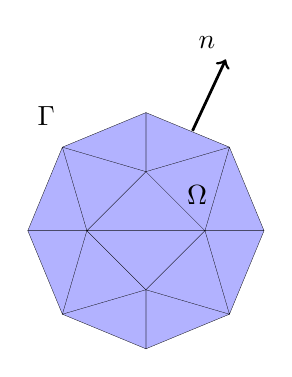
\begin{tikzpicture}
                % FIGURE OF FITTED MESH
                % Boundary points
                \foreach \i in {0, 45, ..., 315} {
                    \coordinate (boundary-\i) at (\i:1.5cm);
                }
                % Interior points
                \coordinate (interior-1) at (0.75, 0);
                \coordinate (interior-2) at (-0.75, 0);
                \coordinate (interior-3) at (0, 0.75);
                \coordinate (interior-4) at (0, -0.75);

                % Create a cycle connecting all the boundary points
                \fill[blue!30] (boundary-0) -- (boundary-45) -- (boundary-90) -- (boundary-135) -- (boundary-180) -- (boundary-225) -- (boundary-270) -- (boundary-315) -- cycle;

                % Labels
                \node[below right] at (0.4,0.7) {$\Omega $};
                \node[below right] at (-1.5,1.7) {$\Gamma $};

                % Triangulation (manually specified)
                \draw[line width=0.1pt] (boundary-0) -- (boundary-45) -- (interior-1) -- cycle;
                \draw[line width=0.1pt] (boundary-45) -- (boundary-90) -- (interior-3) -- cycle;
                \draw[line width=0.1pt] (boundary-90) -- (boundary-135) -- (interior-3) -- cycle;
                \draw[line width=0.1pt] (boundary-135) -- (boundary-180) -- (interior-2) -- cycle;
                \draw[line width=0.1pt] (boundary-180) -- (boundary-225) -- (interior-2) -- cycle;
                \draw[line width=0.1pt] (boundary-225) -- (boundary-270) -- (interior-4) -- cycle;
                \draw[line width=0.1pt] (boundary-270) -- (boundary-315) -- (interior-4) -- cycle;
                \draw[line width=0.1pt] (boundary-315) -- (boundary-0) -- (interior-1) -- cycle;

                % Triangulation between interior points
                \draw[line width=0.1pt] (interior-1) -- (interior-2) -- (interior-3) -- cycle;
                \draw[line width=0.1pt] (interior-1) -- (interior-2) -- (interior-4) -- cycle;

                \draw[->, line width=1.0pt] ({1.4*cos(65)}, { 1.4*sin(65) }) -- ({ 2.4*cos(65)  }, { 2.4*sin(65)  }) node[ above left] {$n $};

            \end{tikzpicture}
            \caption{ Illustration of the mesh $\Omega_{h} $, the boundary $\Gamma $ and the normal vector $n$. }
            \label{fig:domain_construction}
        \end{figure}
    \end{columns}
\end{frame}



\begin{frame}
\frametitle{ $C^0$ Interior Penalty Method (CIP) for the Biharmonic Problem }

\begin{block}{}
    Define the polynomial space \begin{equation}
        V_{h} = \left\{ w \in C^{0}( \Omega )  \mid    w \in  \mathcal{P}_{k}  \right\}
    \end{equation}
The proposed numerical scheme is to find an  $w \in V_{h}$ .t.
\begin{equation*}
a_{h}( w, v )   = l_{h}( v) = ( f,v)_{\Omega } , \quad \forall v \in V_{h}  .
\end{equation*}
where
\begin{equation*}
\begin{split}
a_{h} \left( w, v \right)   =&
    \left( \alpha  w, v \right) _{\Omega }   +  \left( \Delta  w, \Delta v \right) _{\Omega } \\
 & +
  \left( \mean{  \Delta  w }, \jump{ \partial _{n }v} \right)_{\mathcal{F}_{h}}  +
 \left( \mean{ \Delta  v }, \jump{ \partial _{n}w }      \right)_{\mathcal{F}_{h}}  + \frac{\gamma }{h}  \left( \jump{ \partial _{n} w}, \jump{ \partial _{n} v   }   \right)_{\mathcal{F}_{h}}
 % l_{h}( v_{h}) & =  \left( f, v \right) _{\Omega }
\end{split}
\end{equation*}


\end{block}

% \footnotetext[1]{\fullcite{brenner2012}}

\end{frame}


\begin{frame}
\frametitle{Cut Finite Element Method (CutFEM)}

\begin{block}{Unfitted mesh vs fitted mesh}
    CutFEM is a numerical method for solving partial differential equations (PDEs) using an unfitted mesh.

\begin{figure}
    \centering
    % First TikZ picture
    \begin{minipage}{0.45\textwidth}
        \centering
        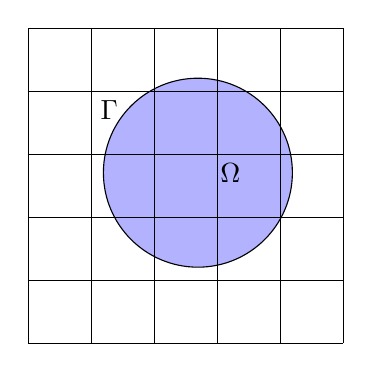
\begin{tikzpicture}[scale=0.80]
            \draw[fill=blue!30] (0.2, 0.2) circle (1.5cm);
            % Background mesh
            \foreach \i in {-2.5, -1.5, ..., 2.5} {
                \draw[line width=0.1pt, shift={(-2.5,\i)}] (0,0) -- (5,0);
                \draw[line width=0.1pt, shift={(\i,-2.5)}] (0,0) -- (0,5);
            }
            % Labels
            \node[below right] at (0.4,0.5) {$\Omega $};
            \node[below right] at (-1.5,1.5) {$\Gamma $};
            % \draw[blue, thick] (-2.5, -2.5) rectangle (2.5, 2.5);
        \end{tikzpicture}
    \end{minipage}
    \hfill
    % Second TikZ picture
    \begin{minipage}{0.45\textwidth}
        \centering
        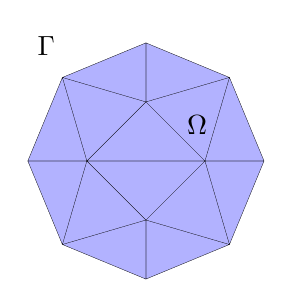
\begin{tikzpicture}[scale=1.0]
            % FIGURE OF UNFITTED MESH
            % Boundary points
            \foreach \i in {0, 45, ..., 315} {
                \coordinate (boundary-\i) at (\i:1.5cm);
            }
            % Interior points
            \coordinate (interior-1) at (0.75, 0);
            \coordinate (interior-2) at (-0.75, 0);
            \coordinate (interior-3) at (0, 0.75);
            \coordinate (interior-4) at (0, -0.75);

            % Create a cycle connecting all the boundary points
            \fill[blue!30] (boundary-0) -- (boundary-45) -- (boundary-90) -- (boundary-135) -- (boundary-180) -- (boundary-225) -- (boundary-270) -- (boundary-315) -- cycle;

            % Labels
            \node[below right] at (0.4,0.7) {$\Omega $};
            \node[below right] at (-1.5,1.7) {$\Gamma $};

            % Triangulation (manually specified)
            \draw[line width=0.1pt] (boundary-0) -- (boundary-45) -- (interior-1) -- cycle;
            \draw[line width=0.1pt] (boundary-45) -- (boundary-90) -- (interior-3) -- cycle;
            \draw[line width=0.1pt] (boundary-90) -- (boundary-135) -- (interior-3) -- cycle;
            \draw[line width=0.1pt] (boundary-135) -- (boundary-180) -- (interior-2) -- cycle;
            \draw[line width=0.1pt] (boundary-180) -- (boundary-225) -- (interior-2) -- cycle;
            \draw[line width=0.1pt] (boundary-225) -- (boundary-270) -- (interior-4) -- cycle;
            \draw[line width=0.1pt] (boundary-270) -- (boundary-315) -- (interior-4) -- cycle;
            \draw[line width=0.1pt] (boundary-315) -- (boundary-0) -- (interior-1) -- cycle;

            % Triangulation between interior points
            \draw[line width=0.1pt] (interior-1) -- (interior-2) -- (interior-3) -- cycle;
            \draw[line width=0.1pt] (interior-1) -- (interior-2) -- (interior-4) -- cycle;

            % \draw[blue, thick] (-2.5, -2.5) rectangle (2.5, 2.5);

        \end{tikzpicture}
    \end{minipage}


    % \caption{Mesh comparison: unfitted mesh (left) adheres to domain and boundary, while fitted mesh (right) employs a triangular mesh for polygonal approximation of the circular domain.}
    \label{fig:domain_mesh}
    \end{figure}
\end{block}

\end{frame}


\begin{frame}
    \frametitle{Cut Finite Element Method}
    \begin{columns}
        % Left column
        \begin{column}{0.5\textwidth}
            Interior Mesh and Cut Cells
            \begin{block}{}
                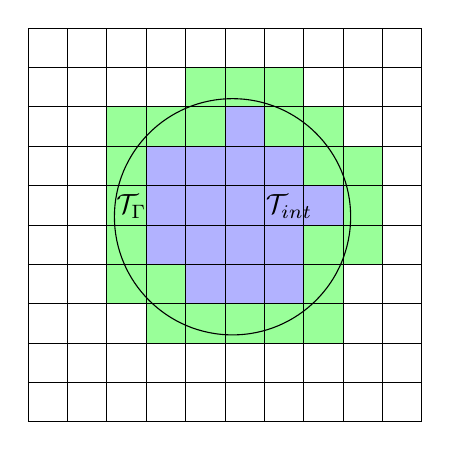
\begin{tikzpicture}[scale=1]
                    % POTENTIAL ACTIVE MESH
                    \fill[blue!30] (2,2) -- (2,-1.5) --(-1.5,-1.5) -- (-1.5,2) -- cycle;

                    % ELEMENTS WITH NO INTERSECTION
                    % lower left
                    \fill[white] (-1.5,-1.5) rectangle (-1.0,-1.0);
                    \fill[white] (-1.5,2.0) rectangle (-1.0,1.5);
                    \fill[white] (-1.0,2.0) rectangle (-0.5,1.5);
                    \fill[white] (2,2) rectangle (1.5,1.5);
                    \fill[white] (1.5,2) rectangle (1.0,1.5);
                    \fill[white] (2,1.5) rectangle (1.5,1.0);
                    \fill[white] (1.5,-1) rectangle (2,-1.5);
                    \fill[white] (1.5,-0.5) rectangle (2,-1.0);

                    % CUT ELEMENTS
                    \fill[green!40] (-0.5,2.0) rectangle (1.0,1.5);
                    \fill[green!40] (-1.5,1.5) rectangle (0.0,1.0);
                    \fill[green!40] (0.5,1.5) rectangle (1.5,1.0);
                    \fill[green!40] (-1.5,1.0) rectangle (-1.0,-1.0);
                    \fill[green!40] (-1.0,-0.5) rectangle (-0.5,-1.5);
                    \fill[green!40] (-0.5,-1.5) rectangle (1.5,-1.0);
                    \fill[green!40] (1.5,-1) rectangle (1.0,-0.0);
                    \fill[green!40] (1.5,-0.5) rectangle (2.0,1.0);
                    \fill[green!40] (1.0,0.5) rectangle (1.5,1.0);

                    \draw (0.1, 0.1) circle (1.5cm);
                    % Background mesh
                    \foreach \i in {-2.5, -2, ..., 2.5} {
                        \draw[line width=0.1pt, shift={(-2.5,\i)}] (0,0) -- (5,0);
                        \draw[line width=0.1pt, shift={(\i,-2.5)}] (0,0) -- (0,5);
                    }

                    % Labels
                    \node[below right] at (0.4,0.5) {$\mathcal{T}_{\text{int}}$};
                    \node[below right] at (-1.5,0.5) {$\mathcal{T}_{\Gamma}$};
                \end{tikzpicture}
            \end{block}
        \end{column}
        % Right column
        \begin{column}{0.5\textwidth}
            \begin{block}{}
                \begin{itemize}
                    \item Adding a regularization term to ensure well-posedness.
\begin{equation*}
    A_h(w,v) = a_{h}(w, v) + \textcolor{red}{g(w, v)} = l( v)
\end{equation*}
                    \item Efficient handling of complex and moving domains.
                \end{itemize}
            \end{block}
        \end{column}
    \end{columns}
\end{frame}



\begin{frame}
\frametitle{Recall the Cahn Hilliard Equation}
    \begin{columns}
        % Left column
        \begin{column}{0.5\textwidth}
            \begin{block}{Recall}
                The problem has the form $u( x, t): \Omega \times [0,T] \mapsto [-1,1]$ and $u(0,x)  =u_0$ s.t.
                \[
                \begin{split}
                    u_t+\Delta\left(\varepsilon ^2 \Delta u- f(u)\right)&= g_0(x,t) \quad \text{in } \Omega \\
                    \partial_n u & =g_1(x,t) \quad \text{on } \Gamma  \\
                    \partial_n \Delta u& =g_2(x,t) \quad \text{on } \Gamma  \\
                \end{split}
                \]
                where $f(u)$ is a nonlinear function.
            \end{block}
        \end{column}
        % Right column
        \begin{column}{0.5\textwidth}
            \begin{block}{Plan forward}
                \begin{enumerate}
                    \item We have now a tool to solve the $\Delta ( \Delta u) $ operator
                    \item Will utilize the time-iteration scheme to solve non-linearity
                \end{enumerate}
            \end{block}
        \end{column}
    \end{columns}
\end{frame}




\begin{frame}
\frametitle{The CutCIP Cahn-Hilliard Formulation}


\begin{block}{IMEX method on the CutCIP formulation}
    Let $u^{m}_{h} \in V_{h}$ for the timesteps $m=0,1,\ldots,M$. Let $u_{h}^{0} = u_{0}$ be the initial timestep, then is.
\begin{equation}
( \overline{\partial } _{t} u^{m}_{h}, v_{h}   )_{\Omega } + \varepsilon^{2} A^{}_{h}( u_{h}^{m} , v) +  c_{h} (  u_{h}^{m-1}, v_{h})  = \varepsilon ^2 l_{h}^{}( v_{h})  , \quad \forall v_{h}, u^{m}_{h} \in V^{}_{h}.
\end{equation}
Here is $c_{h}( . , .) $ an the nonlinear terms handled in a implicit fashion. The $ \overline{\partial}  _{t}$ operator is simply a finite difference scheme in time-dimension.

\end{block}

\footnotetext[1]{\fullcite{feng2007fully}}
\end{frame}

\begin{frame}
\frametitle{ Cut $C^0$ Interior Penalty Method Results }
% \frametitle{Manufactured Solution}

\begin{block}{Manufactured solution}
For our experiment we chose the manufactured solution
\begin{equation}
    u_{ ex }(x, t) = \sin\left(\frac{2\pi x_1}{\sqrt{\varepsilon}}\right)\cos\left(\frac{2 \pi x_2}{\sqrt{\varepsilon}}\right)\cos\left(\frac{2\pi t}{\varepsilon^2}\right)\exp\left(-\frac{t}{\varepsilon^2}\right)
\end{equation}
This manufactured solution can be used to test the accuracy of numerical methods for solving the above differential equation.
\end{block}
\end{frame}


\begin{frame}
\frametitle{Convergence results}
\begin{figure}[h]
    \centering
    \includegraphics[width=0.7\textwidth]{CH-example/spatial-plot.pdf}
\end{figure}
\end{frame}


\begin{frame}
\frametitle{The CutCIP Cahn-Hilliard Experiments}
\begin{center}
    \begin{tabular}{ccc}
        \includegraphics[width=0.2\textwidth]{CH-example/flower_0.png} &
        \includegraphics[width=0.2\textwidth]{CH-example/flower_10.png} &
        \includegraphics[width=0.2\textwidth]{CH-example/flower_50.png} \\
        Step 0 & Step 10 & Step 50 \\
        \includegraphics[width=0.2\textwidth]{CH-example/flower_200.png} &
        \includegraphics[width=0.2\textwidth]{CH-example/flower_500.png} &
        \includegraphics[width=0.2\textwidth]{CH-example/flower_1000.png} \\
        Step 200 & Step 500 & Step 1000 \\
    \end{tabular}
\end{center}
\end{frame}


\begin{frame}
\frametitle{The CutCIP Cahn-Hilliard Experiments}
\begin{center}
    \begin{tabular}{ccc}
        \includegraphics[width=0.2\textwidth]{CH-example/popcorn_0.png} &
        \includegraphics[width=0.2\textwidth]{CH-example/popcorn_10.png} &
        \includegraphics[width=0.2\textwidth]{CH-example/popcorn_50.png} \\
        Step 0 & Step 10 & Step 50 \\
        \includegraphics[width=0.2\textwidth]{CH-example/popcorn_200.png} &
        \includegraphics[width=0.2\textwidth]{CH-example/popcorn_500.png} &
        \includegraphics[width=0.2\textwidth]{CH-example/popcorn_1000.png} \\
        Step 200 & Step 500 & Step 1000 \\
    \end{tabular}
\end{center}
\end{frame}


\begin{frame}
\frametitle{Questions?}
\end{frame}

\begin{frame}
\begin{center}
\begin{columns}
\begin{column}{0.5\textwidth}
    \textbf{Energy Functional:}
    \begin{equation*}
        E(u) = \int_{\Omega} \left( \frac{\varepsilon^2}{2} |\nabla u|^2 + F(u) \right) \, dx.
    \end{equation*}
    Decomposing \( E(u) \) into:
    \begin{align*}
        E_{1}(u) &= \int_{\Omega} \frac{\varepsilon^2}{2} |\nabla u|^2 \, dx, \text{ (smoothness)} \\
        E_{2}(u) &= \int_{\Omega} F(u) \, dx \text{ (separation)}.
    \end{align*}
    For chemical energy \( F(s)=\frac{1}{4}\left(s^2-1\right)^2 \)
\end{column}
\begin{column}{0.5\textwidth}
    \textbf{Physical Expectations:}
    \begin{equation*}
        \frac{d}{dt} E(u) < 0, \quad \frac{d}{dt} \int_{\Omega} u \, dx = 0.
    \end{equation*}
\end{column}
\end{columns}
\end{center}
\end{frame}

\begin{frame}
\begin{center}
    \includegraphics[width=1.0\textwidth]{CH-example/physical_energy.pdf}
\end{center}
\end{frame}


